\documentclass[10pt]{article}
\usepackage[ngerman]{babel}
\usepackage[utf8]{inputenc}
\usepackage[T1]{fontenc}
\usepackage{graphicx}
\usepackage[export]{adjustbox}
\graphicspath{ {./images/} }
\usepackage{amsmath}
\usepackage{amsfonts}
\usepackage{amssymb}
\usepackage[version=4]{mhchem}
\usepackage{stmaryrd}

\title{Bachelor of Science (BSc) in Informatik Modul Software-Entwicklung 1 (SWEN1) }

\author{}
\date{}


\begin{document}
\maketitle
\section*{LE 06 - Softwarearchitektur und Design II}
SWEN1/PM3 Team:\\
R. Ferri (feit), D. Liebhart (lieh), K. Bleisch (bles), G. Wyder (wydg)

\section*{Um was geht es?}
\begin{itemize}
  \item Wie realisiere ich einen Use Case mit Klassen, die klare Verantwortlichkeiten haben, wartbar und einfach erweiterbar sind?
  \item Wie modelliere ich mein Design mit der UML, um es diskutieren und evaluieren zu können?\\
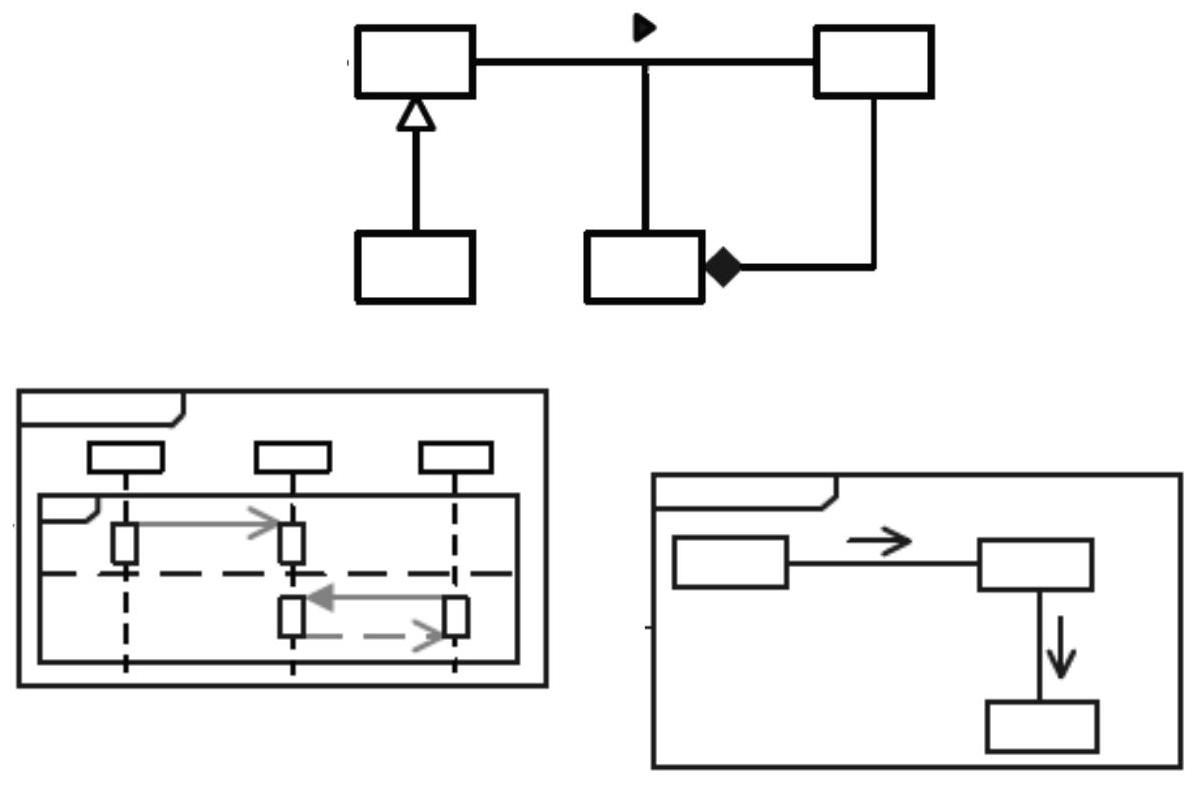
\includegraphics[max width=\textwidth, center]{2025_01_02_787afb9584031d2940deg-02}
\end{itemize}

\section*{Lernziele LE 06 - Softwarearchitektur und Design II}
\begin{itemize}
  \item Sie sind in der Lage:
  \item den Zweck und die Anwendung von statischen und dynamischen Modellen im Design zu erläutern,
  \item einen Objektentwurf zweckmässig mit UML-Klassen-, UML-Interaktions-, UML-Zustands- und UML-Aktivitätsdiagrammen darzustellen.
  \item die Idee von Verantwortlichkeiten und des Responsibility-Driven Designs (RDD) für den Entwurf von Klassen zu erklären,
  \item grundlegende Prinzipen und Pattern für den Klassenentwurf anzuwenden (GRASP, SOLID),
\end{itemize}

\begin{enumerate}
  \item Einführung in das objektorientierte Design
  \item UML-Diagramme für das Design
  \item Klassen mit Verantwortlichkeiten entwerfen
  \item Wrap-up und Ausblick
\end{enumerate}

\section*{Recap: Objektorientierung}
\begin{itemize}
  \item Was bedeutet Objektorientierung?
\end{itemize}

\section*{Recap: Objektorientierte Analyse und objektorientiertes Design}
\begin{center}
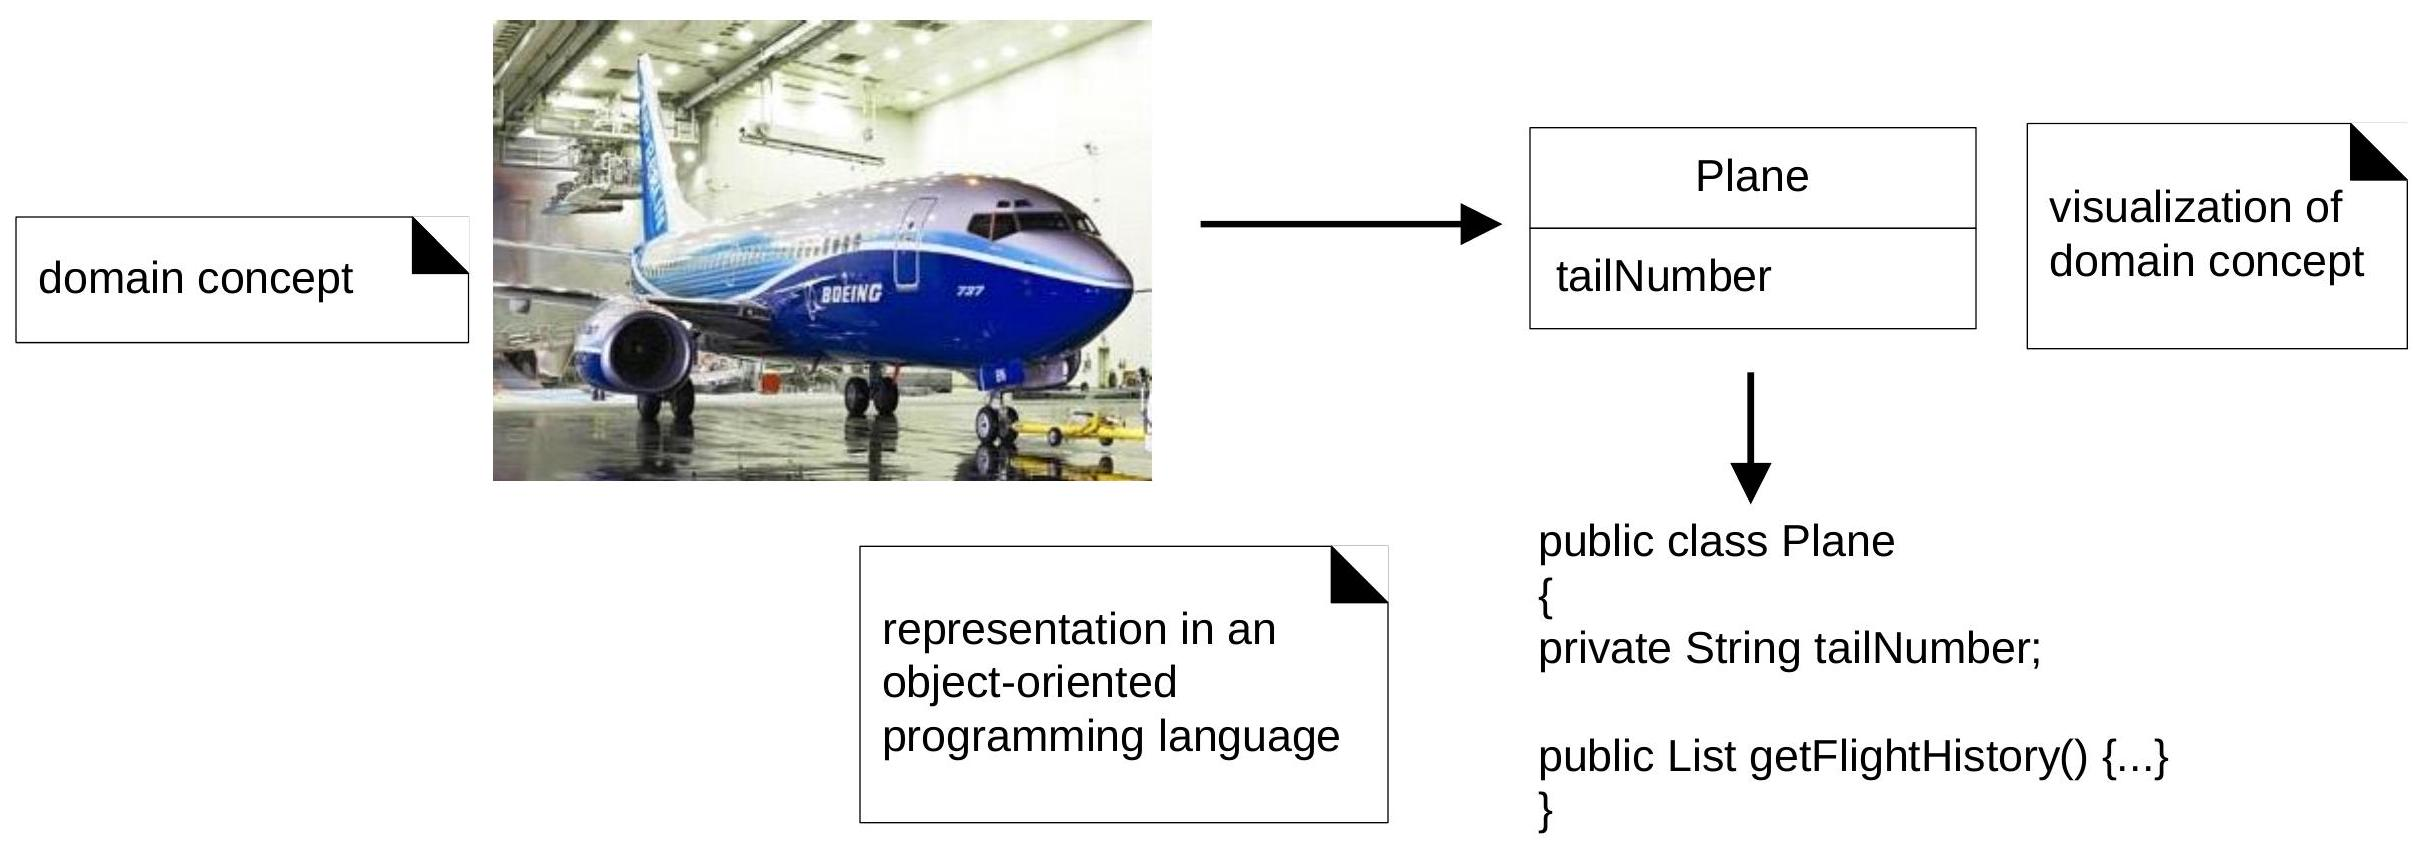
\includegraphics[max width=\textwidth]{2025_01_02_787afb9584031d2940deg-06}
\end{center}

\section*{Use Cases und System-Sequenzdiagramm (SSD)}
\begin{itemize}
  \item Szenarien und
\end{itemize}

Systemoperationen, die in den\\
Use Cases identifiziert wurden, zusammen mit dem Domänenmodell bilden die Basis für das Design.

\begin{itemize}
  \item Die Systemoperation bzw. deren Antworten sind schlussendlich das, was programmiert werden muss.\\
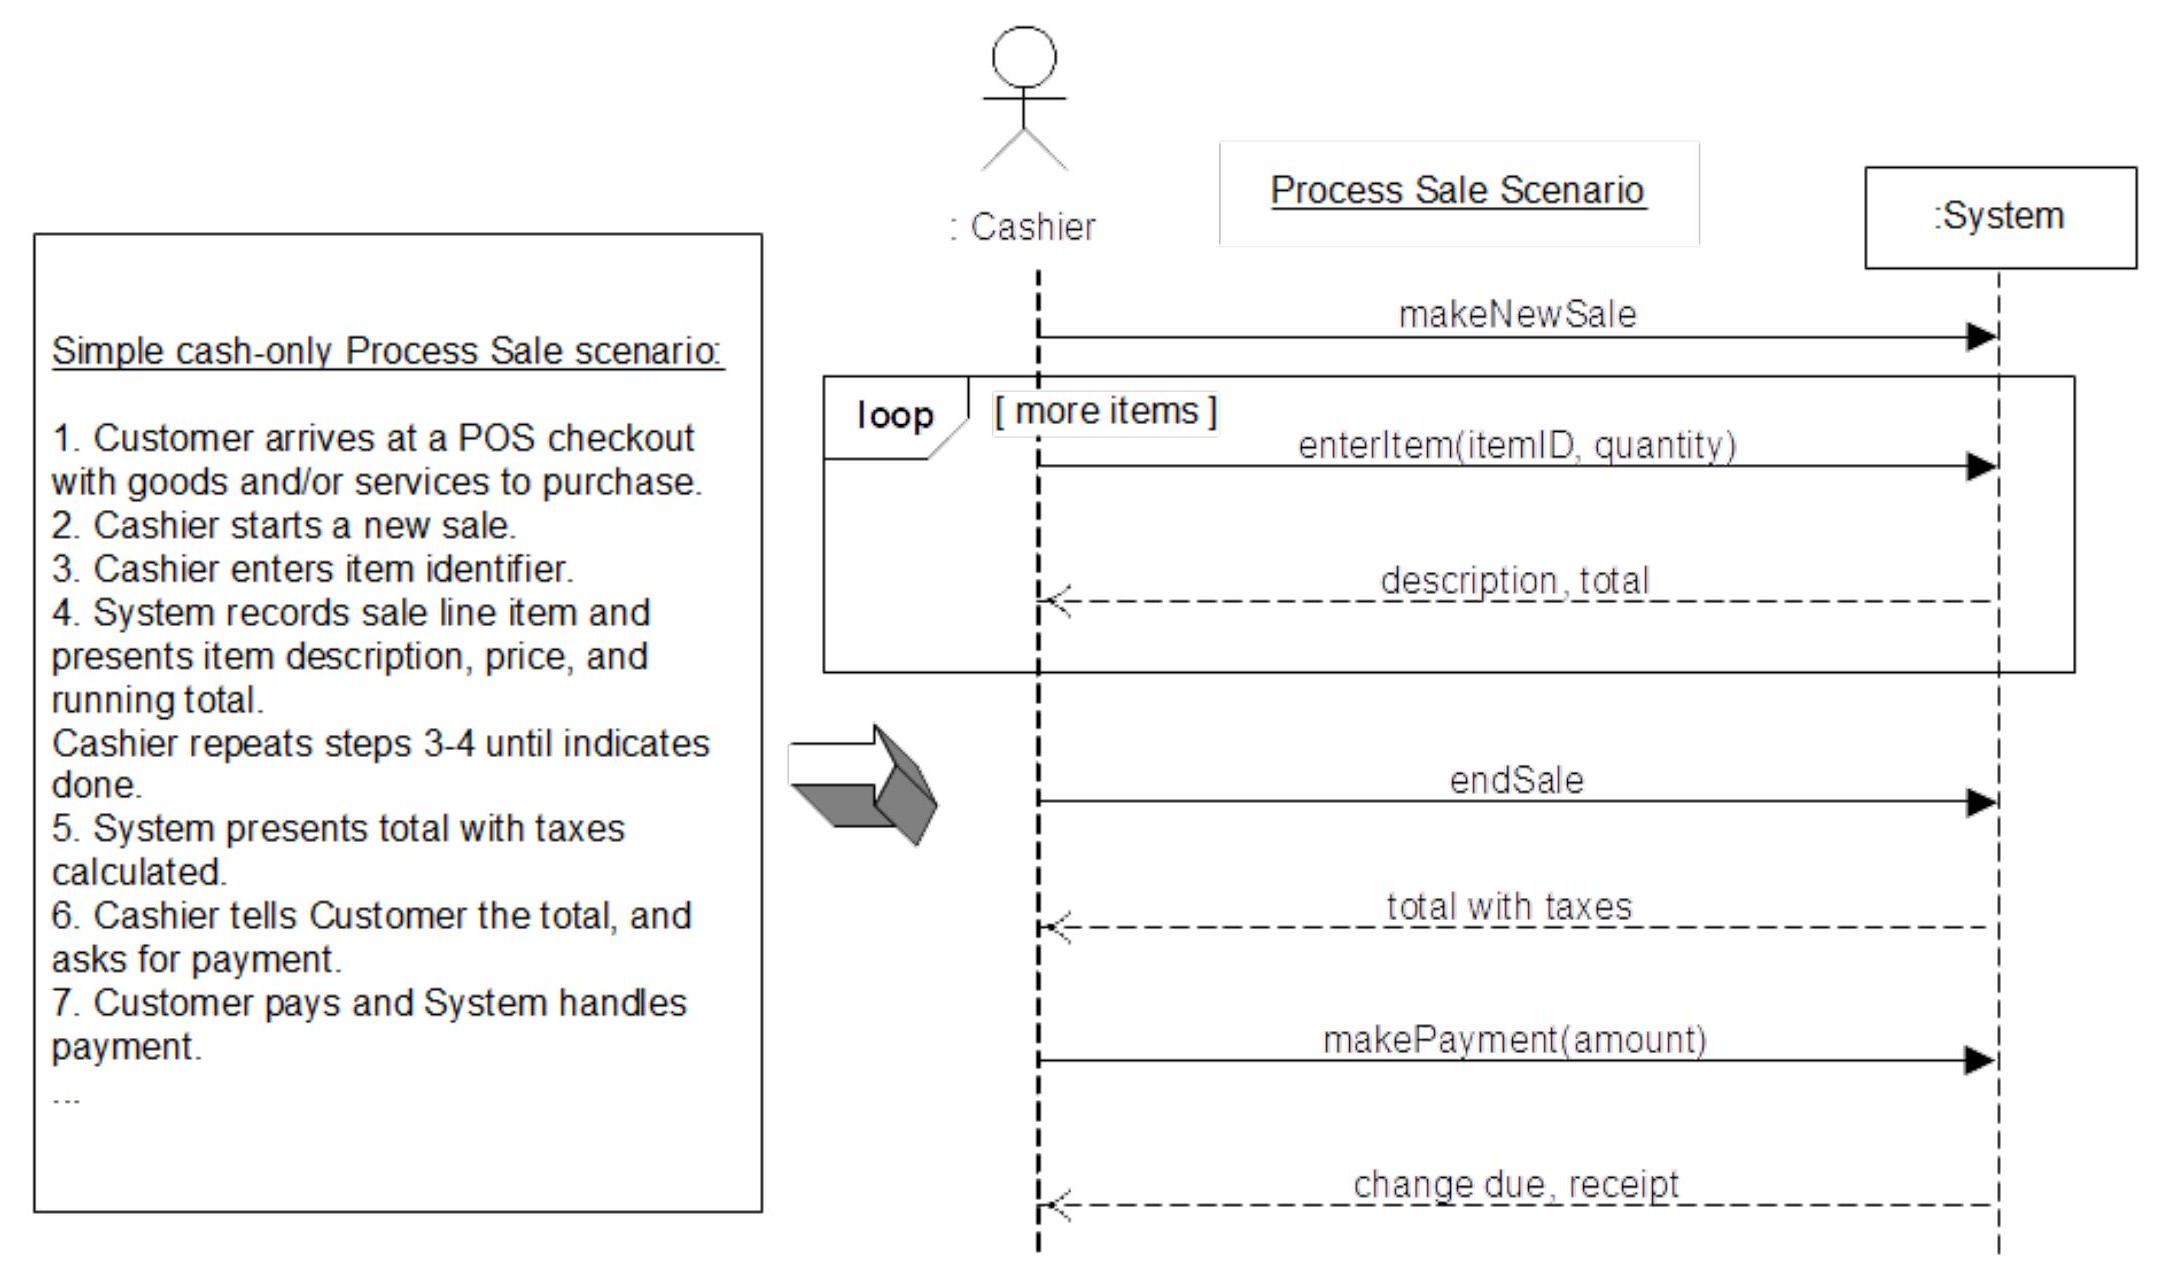
\includegraphics[max width=\textwidth, center]{2025_01_02_787afb9584031d2940deg-07}
\end{itemize}

\section*{Use Cases und Use-Case-Realisierung}
\begin{itemize}
  \item Eine Use-Case-Realisierung beschreibt, wie ein bestimmter Use Case innerhalb des Designs mit kollaborierenden Objekten realisiert wird.
  \item Jedes Szenario eines Use Cases bzw. dessen Systemoperationen werden schrittweise entworfen und implementiert.
  \item Die UML-Diagramme sind eine gemeinsame Sprache, um Use-Case-Realisierungen zu veranschaulichen und zu diskutieren.
\end{itemize}

\section*{Klassen entwerfen: \\
 Statische und dynamische Modellierung}
\begin{itemize}
  \item Es gibt zwei Arten von Design-Modellen:
  \item Statische Modelle
  \item Statische Modelle, wie beispielsweise das UML-Klassendiagramm, unterstützen den Entwurf von Paketen, Klassennamen, Attributen und Methodensignaturen (ohne Methodenkörper).
  \item Dynamische Modelle
  \item Dynamische Modelle, wie beispielsweise UMLInteraktionsdiagramme, unterstützten den Entwurf der Logik, des\\
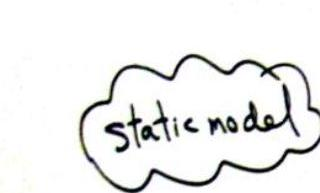
\includegraphics[max width=\textwidth]{2025_01_02_787afb9584031d2940deg-09} Verhaltens des Codes und der Methodenkörper.
  \item Statische und dynamische Modelle ergänzen sich.
  \item Statische und dynamische Modelle werden parallel erstellt.
\end{itemize}

\begin{enumerate}
  \item Einführung in das objektorientierte Design
  \item UML-Diagramme für das Design
  \item Klassen mit Verantwortlichkeiten entwerfen
  \item Wrap-up und Ausblick
\end{enumerate}

\section*{Die Diagramme der UML}

\includegraphics[max width=\textwidth, center]{2025_01_02_787afb9584031d2940deg-11}\\
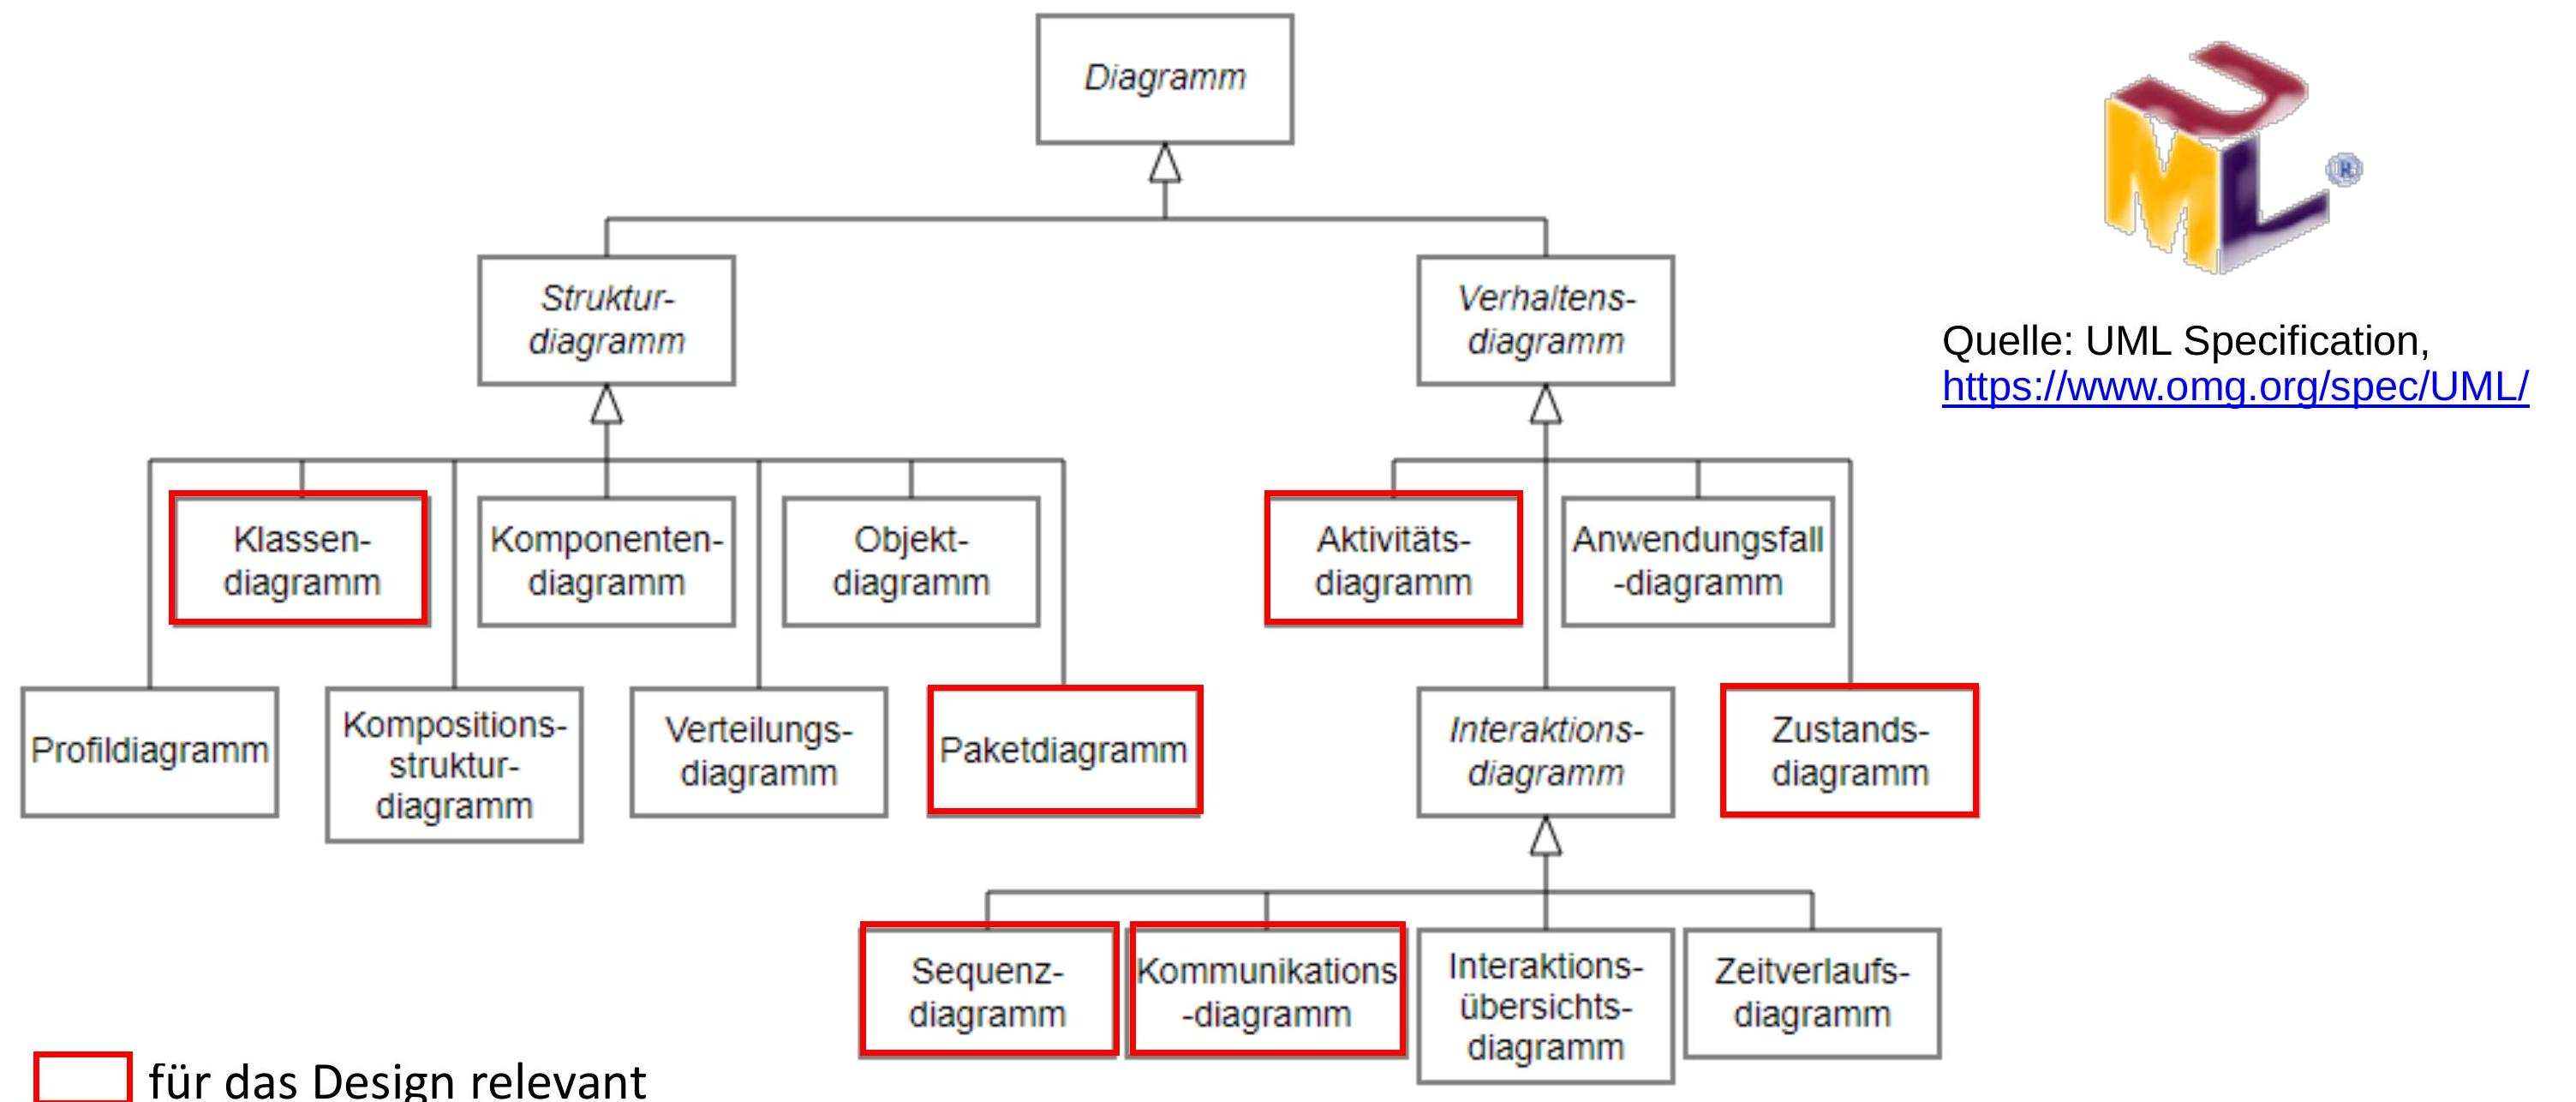
\includegraphics[max width=\textwidth, center]{2025_01_02_787afb9584031d2940deg-11(1)}

\section*{Grundelemente der UML}
School of Engineering

\begin{itemize}
  \item Grundlegende Notationselemente:
  \item Primitiver Datentyp
  \item Literal
  \item Schlüsselwort, Stereotyp
  \item Randbedingung (constraint)
  \item Kommentar
  \item Diagrammrahmen (optional)
\end{itemize}

Optionaler Diagrammrahmen mit\\
Rahmenkürzel und $N$ amen für Diagramme: Rahmenkult\\
aktivity act\\
aktivity act\\
class nichts oder cd\\
component cmp\\
deployment dep\\
package pkg\\
package pkg\\
state machine stm\\
interaction sd\\
use Case uc\\
use Case uc

Ein Stereotyp gibt dem Modell-\\
element eine bestimmte Semantik

Eine Randbedingung (Constraint)\\
kann an jedes Modellelement\\
angefügt werden (auch in\\
Kommentaren),\\
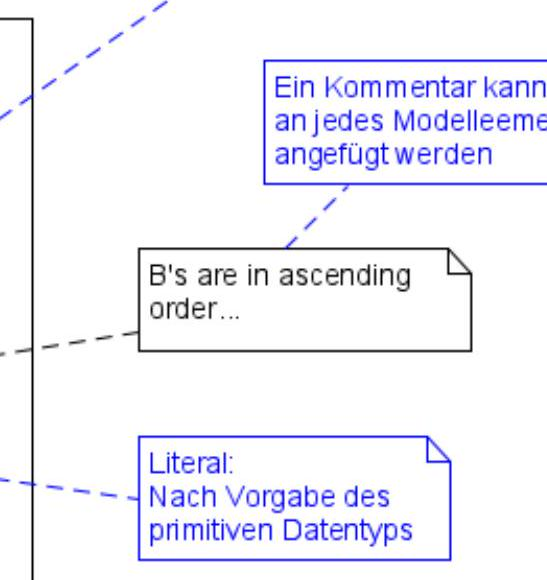
\includegraphics[max width=\textwidth, center]{2025_01_02_787afb9584031d2940deg-12}

Vordefinierte primitive Datentypen in UML: Boolean, Integer, UnlimitedNatural und String. Für Implentati onsprache Java: boolean, byte, short, int, long, float, double, String,\\
Eigene Datentypen und Enumarations w erden beim Klassendiagramm diskutiert

\begin{itemize}
  \item Das Diagramm beantwortet die zentrale Frage: Aus welchen Klassen besteht mein System und wie sind sie miteinander verknüpft?
  \item Es beschreibt die statische Struktur des zu entwerfenden oder abzubildenden Systems.
  \item Welche Klassen und Objekte existieren im System
  \item Welche Attribute, Operationen und Beziehungen haben sie untereinander
  \item Es enthält alle relevanten Strukturzusammenhänge und Datentypen.
  \item Es bildet die Brücke zwischen den dynamischen Diagrammen.
  \item Das UML-Klassendiagramm kann für mehrere Zwecke verwendet werden:
  \item In der Konzeptphase als Domänenmodell mit einem vereinfachten UMLKlassendiagramm (Problemdomäne).
  \item In der Designphase als Design-Klassendiagramm (DCD) mit zusätzlichen Notationselementen (Lösungsdomäne).
\end{itemize}

\section*{UML-Interaktionsdiagramme}
\begin{itemize}
  \item Ein Interaktionsdiagramm spezifiziert, auf welche Weise Nachrichten und Daten zwischen Interaktionspartnern ausgetauscht werden.
  \item Es gibt zwei Arten von UML-Interaktionsdiagrammen:
  \item Sequenzdiagramm
  \item Kommunikationsdiagramm\\
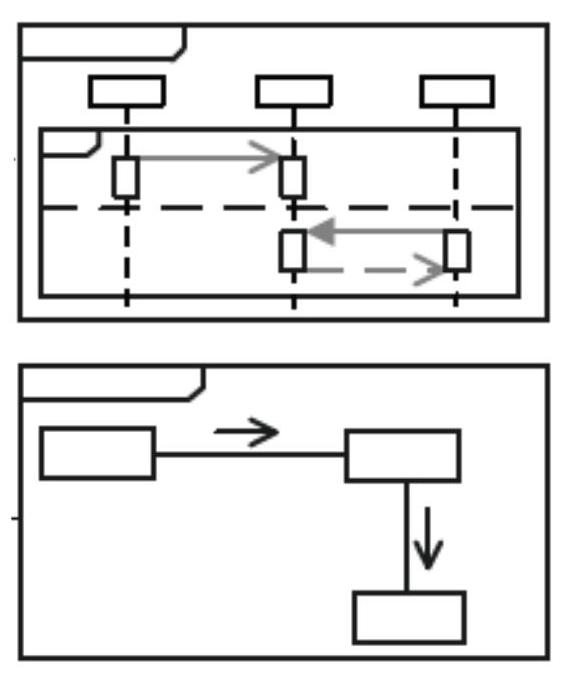
\includegraphics[max width=\textwidth, center]{2025_01_02_787afb9584031d2940deg-14}
  \item Modellieren die Kollaborationen bzw. den Informationsaustausch zwischen Objekten (Dynamik).
\end{itemize}

\section*{UML-Sequenzdiagramm (1/4)}
\begin{itemize}
  \item Das Diagramm beantwortet die zentrale Frage:
\end{itemize}

Wer tauscht mit wem welche Informationen in welcher Reihenfolge aus?

\begin{itemize}
  \item Es stellt den zeitlichen Ablauf des Informationsaustausches zwischen\\
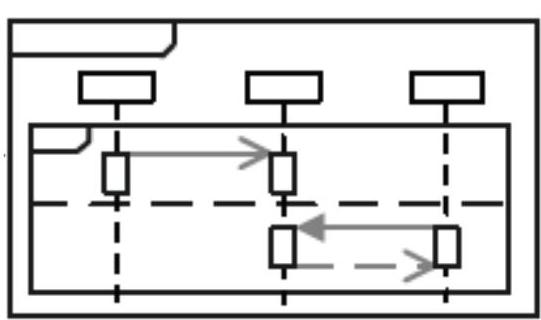
\includegraphics[max width=\textwidth]{2025_01_02_787afb9584031d2940deg-15} Kommunikationspartnern dar.
  \item Es sind Schachtelung und Flusssteuerung (Bedingungen, Schleifen, Verzweigungen) möglich.
\end{itemize}

\section*{UML-Kommunikationsdiagramm (1/3)}
\begin{itemize}
  \item Das Diagramm beantwortet die zentrale Frage:
\end{itemize}

Wer kommuniziert mit wem? Wer «arbeitet» im System zusammen?

\begin{itemize}
  \item Es stellt ebenfalls den Informationsaustausch zwischen Kommunikationspartnern dar.\\
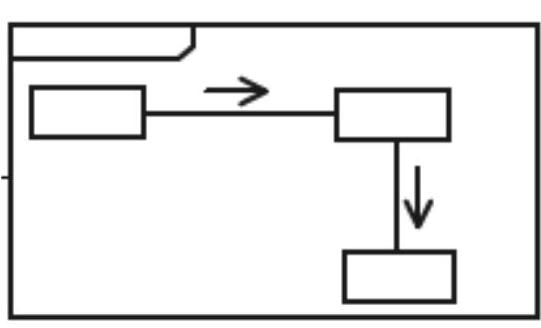
\includegraphics[max width=\textwidth, center]{2025_01_02_787afb9584031d2940deg-16}
  \item Der Überblick steht im Vordergrund (Details und zeitliche Abfolge sind weniger wichtig).
\end{itemize}

\section*{UML-Zustandsdiagramm (1/4)}
\begin{itemize}
  \item Das Diagramm beantwortet die zentrale Frage:
\end{itemize}

Welche Zustände kann ein Objekt, eine Schnittstelle, ein Use Case, ... bei welchen Ereignissen annehmen?

\begin{itemize}
  \item Präzise Abbildung eines Zustandsmodells (endlicher Automat) mit\\
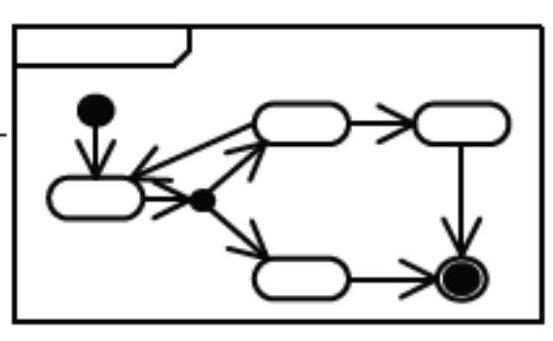
\includegraphics[max width=\textwidth]{2025_01_02_787afb9584031d2940deg-17} Zuständen, Ereignissen, Nebenläufigkeiten, Bedingungen, Ein- und Austrittsaktionen.
  \item Zustände können wieder aus Zuständen bestehen (Schachtelung möglich).
  \item Das Zustandsdiagramm wird vor allem in der Modellierung von Echtzeitsystemen, Steuerungen und Protokollen verwendet.
\end{itemize}

\section*{UML-Aktivitätsdiagramm (1/3)}
\begin{itemize}
  \item Das Diagramm beantwortet die zentrale Frage: Wie läuft ein bestimmter Prozess oder ein Algorithmus ab?
  \item Es kann eine sehr detaillierte Visualisierung von Abläufen mit\\
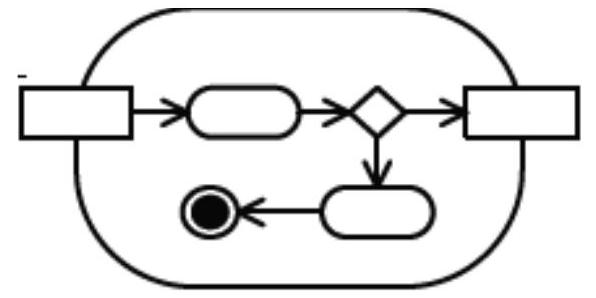
\includegraphics[max width=\textwidth]{2025_01_02_787afb9584031d2940deg-18} Bedingungen, Schleifen und Verzweigungen modelliert werden.
  \item Es sind Parallelisierung und Synchronisation von Aktionen möglich.
\end{itemize}

\section*{Weitere Informationen zur Modellierung mit der UML}
\begin{itemize}
  \item Diese Einführung in die Modellierung mit der UML und in die verschiedenen Diagramme für das Design ist eine kompakte Zusammenfassung, ohne detaillierte Erläuterung der Semantik.
  \item Sie umfasst der wichtigsten Notationselemente, mit denen ca. 80\% der Problemstellungen modelliert werden können.
  \item Achtung: Um damit in der Praxis modellieren zu können, müssen die Diagramme und Notationselemente in verschiedenen Problemstellungen angewendet und eingeübt werden!
\end{itemize}

\section*{Tipps zur Modellierung}
\begin{center}

\includegraphics[max width=\textwidth]{2025_01_02_787afb9584031d2940deg-20}
\end{center}

\begin{itemize}
  \item Modellieren-im-Team: Skizzieren Sie erste Versionen im Team am Whiteboard. Verzichten Sie (vorläufig) auf komplexe Grafik- oder UML-Werkzeuge.
  \item Gerade-gut-genug: Vermeiden Sie das Streben nach Vollständigkeit Ihrer Modelle - meistens genügen Ausschnitte oder Teile des Systems für das Verständnis!
  \item Gerade-rechtzeitig: Verzögern Sie die Erstellung der ausgelieferten Dokumentation - es könnten sich ja noch Dinge ändern!
  \item Dokumentieren Sie kontinuierlich. Am Ende der letzten Iteration oder des Projekts können Sie sich nicht mehr an alle relevanten Dinge erinnern.
  \item Diagramm-plus-Text: Ergänzen Sie grafische Modelle um kurze textuelle Erläuterungen. Gute technische Dokumentation kombiniert Bild mit Text!
  \item Halten Sie Modelle möglichst redundanzfrei. Versuchen Sie, benötigte Dokumente aus einer einheitlichen Informations- oder Modellbasis zu generieren.
\end{itemize}

\begin{enumerate}
  \item Einführung in das objektorientierte Design
  \item UML-Diagramme für das Design
  \item Klassen mit Verantwortlichkeiten entwerfen
  \item Wrap-up und Ausblick
\end{enumerate}

\section*{Verantwortlichkeiten und Responsibility-Driven-Design}
\begin{itemize}
  \item Denken in Verantwortlichkeiten, Rollen und Kollaborationsbeziehungen für den Entwurf von Softwareklassen.
  \item Dieser Ansatz ist das Responsibility-Driven-Design (RDD).
  \item Softwareobjekte werden ähnlich wie Personen betrachtet, mit Verantwortlichkeiten und einer Zusammenarbeit mit anderen Personen, um eine Aufgabe zu erledigen.
  \item Verantwortlichkeiten werden durch Attribute und Methoden implementiert.
  \item Evtl. in Zusammenarbeit mit Operationen von anderen Klassen bzw. Objekten.
  \item RDD kann auf jeder Ebene des Designs angewendet werden (Klasse, Komponente, Schicht).
\end{itemize}

\section*{Ausprägungen von Verantwortlichkeiten}
\begin{itemize}
  \item «Doing»-Verantwortlichkeiten (oder Algorithmen, Code)
  \item Selbst etwas tun
  \item Aktionen anderer Objekte anstossen
  \item Aktivitäten anderer Objekte kontrollieren und steuern
  \item «Knowing»-Verantwortlichkeit (oder Daten, Attribute)
  \item Private eingekapselte Daten
  \item Verwandte Objekte kennen
  \item Dinge kennen, die es ableiten oder berechnen kann
  \item Daten/Objekte zur Verfügung stellen, die aus den bekannten Daten/Objekten abgeleitet oder berechnet werden können
\end{itemize}

\section*{GRASP: Ein methodischer Ansatz für das OO-Design}
\begin{itemize}
  \item GRASP (General Responsibility Assignment Software Patterns) bezeichnet eine Menge von grundlegenden Prinzipen bzw. Pattern, mit denen die Zuständigkeit bestimmter Klassen objektorientierter Systeme festgelegt wird.
  \item Sie beschreiben allgemein welche Klassen und Objekte wofür zuständig sein sollten (Verantwortlichkeiten und Kollaborationen).
  \item Diese allgemein anerkannten Regeln wurden von Craig Larman [1] systematisch beschrieben.
  \item Dies erleichtert die Kommunikation zwischen Softwareentwicklern und erleichtert Einsteigern als Lernhilfe das Entwickeln eines Bewusstseins für guten bzw. schlechten Code.
\end{itemize}

\section*{Prinzipien und Pattern}
\begin{itemize}
  \item Ein Prinzip ist in diesem Kontext ein Grundsatz oder Postulat, das zu einem guten objektorientierten Design führen soll.
  \item Ein Pattern ist ein benanntes Problem-Lösungspaar, das in neuen Kontexten angewendet werden kann.
  \item Weitere Design-Patterns siehe Gang-of-Four (GoF)
  \item Oft wiederkehrende Problemstellungen mit detaillierten Lösungsmustern
\end{itemize}

\section*{GRASP - Neun Prinzipien bzw. Patterns}
\begin{itemize}
  \item Information Expert
  \item Creator
  \item Controller
  \item Low Coupling
  \item High Cohesion
  \item Polymorphism
  \item Pure Fabrication
  \item Indirection
  \item Protected Variations
\end{itemize}

\section*{GRASP - Neun Prinzipien bzw. Patterns}
\begin{itemize}
  \item Bitte die Klasse durchnummerieren und Nummer merken
  \item Bilden Sie den Modulo 9 mit Ihrer Nummer
  \item Erarbeiten Sie das/die Pattern/Prinzipien selbständig. Recherchieren Sie!
  \item Wozu wird das Pattern/Prinzip verwendet?
  \item Wie erkenne ich das Pattern/Prinzip?
  \item Wie wende ich das Pattern/Prinzip an?
  \item Zeigen Sie das Pattern/Prinzip in einem UML-Diagramm
\end{itemize}

\section*{GRASP - Neun Prinzipien bzw. Patterns}
\begin{itemize}
  \item Information Expert (0)
  \item Creator (1)
  \item Controller (2)
  \item Low Coupling (3)
  \item High Cohesion (4)
  \item Polymorphism (5)
  \item Pure Fabrication (6)
  \item Indirection (7)
  \item Protected Variations (8)
  \item Alle Experten zu einem Thema finden sich zusammen, sichten die einzelnen Lösungsteile und erarbeiten eine gemeinsame Aussage, die vorgetragen werden kann.
  \item Ein Experte wird bestimmt, das Pattern/Prinzip allen vorzutragen und zu erklären.
\end{itemize}

\begin{enumerate}
  \item Einführung in das objektorientierte Design
  \item UML-Diagramme für das Design
  \item Klassen mit Verantwortlichkeiten entwerfen
  \item Wrap-up und Ausblick
\end{enumerate}

\section*{Wrap-up}
\begin{itemize}
  \item Das wichtigste Ziel des objektorientierten Designs ist es, Klassen mit klaren Verantwortlichkeiten und Kollaborationen zu entwerfen.
  \item Eine Use-Case-Realisierung wird mit einem Design-Klassendiagramm (DCD) und mehreren Interaktionsdiagrammen modelliert, um das Design zu diskutieren und evaluieren zu können.
  \item Dabei werden das Design-Klassendiagramm und die weiteren Modellierungsartefakte schrittweise erweitert und ergänzt durch jedes entworfene und implementierte Use-CaseSzenario.
  \item GRASP ist eine Lernhilfe, um beim Design bewusst die Verantwortlichkeiten und Kollaborationen zwischen Objekten festzulegen.
  \item GRASP sind grundlegende Prinzipien und Patterns, die zu einem guten objektorientierten Design führen und das Design nachvollziehbar begründen.
  \item In der nächsten Lerneinheit werden wir:
  \item wichtige Aspekte für die Implementation einer Use-Case-Realisierung diskutieren.
\end{itemize}

\section*{Quellenverzeichnis}
[1] Larman, C.: UML 2 und Patterns angewendet, mitp Professional, 2005\\[0pt]
[2] Seidel, M. et al.: UML @ Classroom: Eine Einführung in die objektorientierte Modellierung, dpunkt.verlag, 2012\\[0pt]
[3] Martin, R. C.: Clean Architecture: A Craftsman's Guide to Software Structure and Design, mitp Professional, 2018


\end{document}